\documentclass[10pt,twocolumn]{article}

% ---------------------------------------------------------------------------
% LLM-Assisted Generation of Data Quality Constraints from Schema and
% Documentation. Self-contained draft; compiles with tectonic/pdflatex.
% Numbers are drawn verbatim from results/tables/*.csv (medium-scope run).
% ---------------------------------------------------------------------------

\usepackage[margin=0.85in]{geometry}
\usepackage{booktabs}
\usepackage{graphicx}
\usepackage{amsmath}
\usepackage{amssymb}
\usepackage{array}
\usepackage{xcolor}
\usepackage{url}
\usepackage[hidelinks]{hyperref}
\usepackage{caption}
\captionsetup{font=small,labelfont=bf}

\newcommand{\best}[1]{\textbf{#1}}

\title{\vspace{-2em}\textbf{LLM-Assisted Generation of Data Quality Constraints\\
from Schema and Documentation}}
\author{}
\date{}

\begin{document}
\maketitle

\begin{abstract}
Data quality constraints---executable assertions such as ``\texttt{fare\_amount}
is non-negative'' or ``\texttt{o\_orderstatus} $\in \{O,F,P\}$''---are the
backbone of production data pipelines, yet authoring them by hand is slow and
requires both domain and engineering expertise. We ask whether large language
models (LLMs) can draft such constraints directly from a table's schema and
natural-language documentation, and how the resulting suites compare to
traditional baselines. We build an end-to-end, fully reproducible pipeline that
(i) prompts an LLM to emit constraints restricted to a 21-type allowlist of
Great Expectations assertions, (ii) parses and validates every candidate for
executability, and (iii) measures row-level detection against a controlled
error-injection benchmark spanning eight error types over four tables from the
NYC~Taxi and TPC-H datasets. Across three locally served open-weight models we
find that: (RQ1)~executability tracks model scale and code specialization
sharply---a 32B code model reaches 0.90 executability while 7--8B models fall to
0.53--0.58; (RQ2)~classical baselines still lead on raw detection (statistical
profiling recall 0.73, hand-written rules $F_1$ 0.92) but no single method
dominates \emph{per error type}, and the best LLM is the most \emph{balanced}
detector, uniquely covering cross-column logic that profiling misses entirely;
(RQ3)~adding documentation to the prompt is the single largest lever (recall
$0.37\!\to\!0.59$), whereas appending sample rows \emph{hurts}; and (RQ4)~among
local models a 32B code model dominates every axis at a $5$--$7\times$ latency
cost. We release all code, prompts, and the injection benchmark.
\end{abstract}

% ===========================================================================
\section{Introduction}
% ===========================================================================
Modern data pipelines guard themselves with \emph{data quality constraints}:
machine-checkable assertions that a column is non-null, that a categorical field
takes only known values, that a key is unique, or that one timestamp precedes
another. Frameworks such as Great Expectations~\cite{greatexpectations} and
Deequ~\cite{amazondeequ} make such assertions first-class and runnable at scale.
The bottleneck is \emph{authoring}: a human must read the schema, understand the
domain, and translate tacit expectations into concrete, correctly-parameterized
checks. This is laborious, easy to leave incomplete, and rarely revisited.

Large language models are attractive here because the raw ingredients---a
schema and a data dictionary---are exactly the textual context LLMs consume
well, and the target artifact (a list of typed assertions) is close to code.
Recent work shows foundation models can perform data-wrangling tasks such as
entity matching and imputation~\cite{llmdataeng}. We study a narrower, deployable
question: \emph{can an LLM draft a data quality suite from schema and
documentation alone, and is that suite good enough to be useful next to the
baselines a practitioner already has?}

A credible answer has to separate two things that are easy to conflate. First,
\textbf{executability}: do the generated assertions parse, bind to real columns,
and run without error? A suite that reads well but throws at runtime is worthless.
Second, \textbf{detection}: when real errors are present, does the suite flag the
offending rows, and without crying wolf on clean data? We measure both, and we do
so against a \emph{controlled} benchmark---we inject known errors at known rates
and positions, so recall and false-positive rates are ground-truth, not
estimates.

\paragraph{Contributions.}
\begin{itemize}
  \item A reproducible pipeline that turns (schema, docs) into a validated Great
  Expectations suite via an allowlisted prompt, with content-addressed caching
  of all model calls (Section~\ref{sec:approach}).
  \item A controlled error-injection benchmark: eight error types with row-level
  labels over four real tables, plus two classical baselines (statistical
  profiling and hand-written rules) (Section~\ref{sec:setup}).
  \item An empirical study answering four research questions on executability,
  detection vs.\ baselines, prompt context, and local-model choice
  (Section~\ref{sec:results}), with an honest account of where LLMs help and
  where they do not (Section~\ref{sec:discussion}).
\end{itemize}

% ===========================================================================
\section{Research Questions}
% ===========================================================================
\begin{description}
  \item[RQ1 (Executability).] How often do LLM-generated constraints parse,
  bind, and run without error, and how does this depend on the model?
  \item[RQ2 (Detection vs.\ baselines).] How does the detection quality of
  LLM suites (precision/recall/$F_1$, overall and per error type) compare to
  statistical profiling and hand-written rules?
  \item[RQ3 (Prompt context).] What is the effect of enriching the prompt from
  schema only, to schema+documentation, to schema+documentation+sample rows?
  \item[RQ4 (Model choice).] Among locally served open-weight models, how do
  quality and cost trade off?
\end{description}

% ===========================================================================
\section{Approach}\label{sec:approach}
% ===========================================================================
\subsection{From schema and docs to a validated suite}
The pipeline has three stages. \textbf{(1)~Context assembly.} For a target table
we build a prompt containing the column schema (names and inferred types) and,
depending on the experimental condition, a slice of the natural-language data
dictionary and a handful of sample rows. \textbf{(2)~Generation.} The model is
instructed to return a JSON list of assertions drawn from a fixed
\emph{allowlist} of 21 Great Expectations expectation types (e.g.\
\texttt{expect\_column\_values\_to\_not\_be\_null},
\texttt{expect\_column\_values\_to\_be\_in\_set},
\texttt{expect\_column\_pair\_values\_a\_to\_be\_greater\_than\_b}). The allowlist
is the single source of truth shared by the prompt and the parser, which keeps the
output space closed and checkable. \textbf{(3)~Parse and validate.} Each candidate
is parsed and classified as \texttt{valid}, \texttt{json\_error},
\texttt{unknown\_expectation}, or \texttt{invalid\_kwargs}; valid ones are
assembled into a suite and executed with Great Expectations~1.23.2.

Every model call is cached by a content hash of (model, prompt, parameters), so
the entire study is deterministic to re-run and free on cache hits. We decode at
temperature~0.

\subsection{Row-level validation}
To measure detection at row granularity we attach a stable \texttt{\_row\_id} to
every table and run Great Expectations with \texttt{result\_format=COMPLETE} and
\texttt{unexpected\_index\_column\_names=[\_row\_id]}. The union of flagged
\texttt{\_row\_id}s across all expectations in a suite is the set of rows the
suite ``caught,'' which we compare against the injected-error labels. Because
\texttt{COMPLETE} materialization is linear in table size, very large tables are
validated on a fixed-seed uniform subsample for \emph{per-row} error types only;
cross-row error types (duplicates, mixed) are never subsampled, since detecting a
duplicate requires its twin to be present.

\subsection{Baselines}
We compare against two baselines a practitioner would plausibly reach for first.
\textbf{Statistical profiling} learns per-column ranges, null rates, and value
sets from the clean table and emits conservative expectations from them.
\textbf{Hand-written rules} are a small expert suite encoding the documented
integrity constraints (e.g.\ enum domains, non-negativity, key uniqueness,
dropoff-after-pickup). Both are condition-independent and never see injected
errors during authoring.

% ===========================================================================
\section{Experimental Setup}\label{sec:setup}
% ===========================================================================
\subsection{Datasets}
We use four real tables. \textbf{NYC~Taxi} (yellow-cab trip records,
2024-01)~\cite{nyctaxi} is a single wide table sampled to 100k rows after a
documented cleaning pass. \textbf{TPC-H} at scale factor 0.1~\cite{tpch},
generated with DuckDB~\cite{duckdb}, contributes \texttt{orders} (150k),
\texttt{lineitem} (downsampled to 100k with a fixed seed), and \texttt{customer}
(15k), including the \texttt{lineitem}$\to$\texttt{orders}$\to$\texttt{customer}
foreign-key chain. Each table carries a markdown data dictionary used as the
documentation context.

\subsection{Error injection}
We inject eight error types with ground-truth row labels: \emph{missing value},
\emph{out of range}, \emph{type/format error}, \emph{invalid category},
\emph{duplicate row}, \emph{referential integrity} (dangling foreign key),
\emph{cross-column logic} (a documented inter-column relationship violated), and
\emph{distribution shift}. For each table a fixed injection plan targets
appropriate columns. Single-error datasets are produced at corruption rates
$\{0.01, 0.05\}$ with seeds $\{1,2\}$; a ``mixed'' dataset per seed combines all
injectors on disjoint row subsets. This yields 96 single-error corrupted datasets
for recall measurement plus the mixed datasets.

\subsection{Conditions, models, metrics}
The prompt \textbf{conditions} are: \textbf{(a)}~schema only; \textbf{(b)}~schema
+ documentation; \textbf{(c)}~schema + documentation + 10 sample rows. We run three
locally served open-weight \textbf{models} via Ollama~\cite{ollama}:
\texttt{qwen2.5-coder:32b} and \texttt{qwen2.5:7b}~\cite{qwen25}, and
\texttt{llama3.1:8b}~\cite{llama3}, all at temperature~0.

For executability we report the \textbf{executability rate} (fraction of returned
rules that are valid \emph{and} run without a runtime error), the clean-data
\textbf{false-positive rate} over rules and over rows, and \textbf{suite size}.
For detection we report \textbf{precision}, \textbf{recall}, and \textbf{$F_1$}
of flagged rows against injected labels, overall and per error type, averaged
across tables, rates, and seeds. The medium-scope run reported here comprises
6{,}704 metric rows; code, prompts, and data generators are released for exact
reproduction.

% ===========================================================================
\section{Results}\label{sec:results}
% ===========================================================================

\subsection{RQ1: Executability}
Table~\ref{tab:exec} shows executability tracks model scale and code
specialization sharply. The 32B code model produces large suites (16.4 rules)
that run 90\% of the time with low clean-data false positives (9\% of rows). The
7--8B models not only produce smaller suites but a large share do not execute
(0.53--0.58), and \texttt{llama3.1-8b} in particular fires on roughly half of
clean rows---a suite that is actively misleading out of the box. The baselines,
by construction, never false-positive on the clean table.

\begin{table}[t]
\centering\small
\caption{RQ1: Executability and clean-data behavior. ``FP(rows)'' is the fraction
of clean rows flagged. Baselines do not emit LLM rules so executability is
not applicable (---).}
\label{tab:exec}
\begin{tabular}{lrrrr}
\toprule
Method & Exec. & FP(rules) & FP(rows) & Suite \\
\midrule
\texttt{stats}              & ---   & 0.00 & 0.00 & 28.8 \\
\texttt{human}              & ---   & 0.00 & 0.00 & 8.0  \\
\texttt{llm:llama3.1-8b}    & 0.53  & 0.48 & 0.51 & 5.4  \\
\texttt{llm:qwen2.5-7b}     & 0.58  & 0.13 & 0.31 & 9.1  \\
\texttt{llm:qwen2.5-coder-32b} & \best{0.90} & \best{0.11} & \best{0.09} & 16.4 \\
\bottomrule
\end{tabular}
\end{table}

\subsection{RQ2: Detection vs.\ baselines}
Overall (Table~\ref{tab:overall}), classical baselines still lead: statistical
profiling has the highest recall (0.73) and hand-written rules the highest $F_1$
(0.92). The best LLM, \texttt{qwen2.5-coder-32b}, is competitive ($F_1$ 0.67) but
does not overtake either baseline; the smaller models trail badly, dragged down
by the low precision implied by their clean-data false positives.

\begin{table}[t]
\centering\small
\caption{RQ2: Overall detection quality (flagged rows vs.\ injected labels),
averaged across tables, rates, and seeds.}
\label{tab:overall}
\begin{tabular}{lrrr}
\toprule
Method & Precision & Recall & $F_1$ \\
\midrule
\texttt{stats}                 & \best{0.95} & \best{0.73} & 0.87 \\
\texttt{human}                 & 0.88 & 0.54 & \best{0.92} \\
\texttt{llm:qwen2.5-coder-32b} & 0.66 & 0.49 & 0.67 \\
\texttt{llm:qwen2.5-7b}        & 0.17 & 0.36 & 0.20 \\
\texttt{llm:llama3.1-8b}       & 0.03 & 0.45 & 0.05 \\
\bottomrule
\end{tabular}
\end{table}

The overall numbers hide the real story, which is \emph{complementarity}
(Table~\ref{tab:bytype}). No method wins everywhere. Statistical profiling is
near-perfect on range/domain errors (invalid category, out-of-range,
missing value, type/format all $\approx 1.0$) but scores \best{0} on
cross-column logic---a profiler over single columns simply cannot express
``$a > b$.'' Hand-written rules nail the documented relational and enum
constraints (cross-column logic, invalid category, type/format all $1.0$) but
miss distributional and referential errors. The 32B LLM is the most
\emph{balanced} detector: it is the only method that both handles cross-column
logic (0.83, near the human suite) \emph{and} spreads non-trivial recall across
missing values (0.67), invalid categories (0.75), and type/format (1.0). This is
the central finding: the LLM's value is coverage breadth, not single-cell
supremacy.

\begin{table*}[t]
\centering\small
\caption{RQ2: Recall by error type. Best per row in \textbf{bold}. The LLM
column shown is the 32B code model. ``r.i.'' = referential integrity;
``x-col'' = cross-column logic.}
\label{tab:bytype}
\begin{tabular}{lrrrrr}
\toprule
Error type & \texttt{human} & \texttt{llama3.1-8b} & \texttt{qwen2.5-7b} & \texttt{qwen2.5-coder-32b} & \texttt{stats} \\
\midrule
cross-column logic (x-col) & \best{1.00} & 0.19 & 0.29 & 0.83 & 0.00 \\
distribution shift         & 0.00 & \best{0.51} & 0.31 & 0.09 & 0.40 \\
duplicate row              & \best{0.76} & 0.51 & 0.31 & 0.51 & 0.51 \\
invalid category           & \best{1.00} & 0.45 & 0.50 & 0.75 & \best{1.00} \\
missing value              & 0.34 & 0.47 & 0.33 & 0.67 & \best{1.00} \\
out of range               & 0.50 & 0.51 & 0.33 & 0.42 & \best{1.00} \\
referential integrity (r.i.) & 0.01 & 0.52 & 0.13 & 0.00 & \best{1.00} \\
type / format error        & \best{1.00} & 0.00 & \best{1.00} & \best{1.00} & \best{1.00} \\
\bottomrule
\end{tabular}
\end{table*}

Two entries deserve a caveat. Statistical profiling scores 1.0 on
\emph{referential integrity} not because it understands foreign keys---it does
not---but because the injected dangling keys are negative sentinel values that
fall below the learned numeric minimum, so a range check catches them
incidentally. Conversely the single-table LLM and human suites score near zero on
referential integrity because core Great Expectations has no cross-table foreign-key
expectation to emit. We treat these as a measurement artifact of a single-table
setting rather than evidence about reasoning.

\begin{figure}[t]
\centering
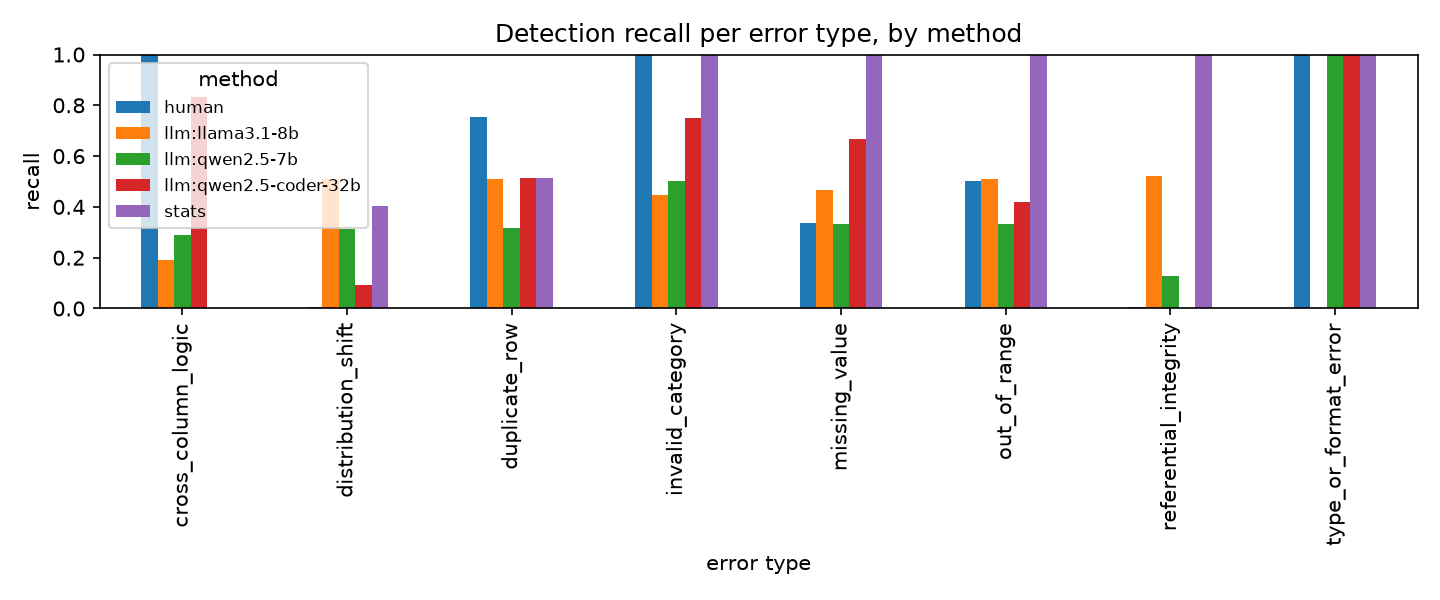
\includegraphics[width=\linewidth]{figures/recall_by_error_type.png}
\caption{Recall by error type across methods (RQ2). No method dominates;
the LLM's profile is the flattest.}
\label{fig:bytype}
\end{figure}

\subsection{RQ3: Prompt context}
Context matters, and not monotonically (Table~\ref{tab:cond}). Moving from schema
only (a) to schema+documentation (b) is the single largest lever in the study:
executability rises $0.67\!\to\!0.81$ and recall $0.37\!\to\!0.59$, as the model
learns enum domains and inter-column relationships it cannot guess from column
names alone, and the mean number of valid rules grows from 8.6 to 13.8. Adding
sample rows (c) \emph{reverses} the gain---executability drops to 0.54 and recall
to 0.33. Inspecting the suites, sample rows lead the model to over-fit to the
specific observed values (e.g.\ narrow numeric bounds or value sets taken from ten
rows), producing brittle assertions that both fail to generalize and misfire. The
practical recommendation is clear: feed documentation, not raw rows.

\begin{table}[t]
\centering\small
\caption{RQ3: Effect of prompt context, averaged over models and tables.}
\label{tab:cond}
\begin{tabular}{llrrr}
\toprule
Cond. & Context & Exec. & Recall & Valid rules \\
\midrule
a & schema            & 0.67 & 0.37 & 8.6 \\
b & +\,documentation  & \best{0.81} & \best{0.59} & 13.8 \\
c & +\,sample rows    & 0.54 & 0.33 & 8.4 \\
\bottomrule
\end{tabular}
\end{table}

\begin{figure}[t]
\centering
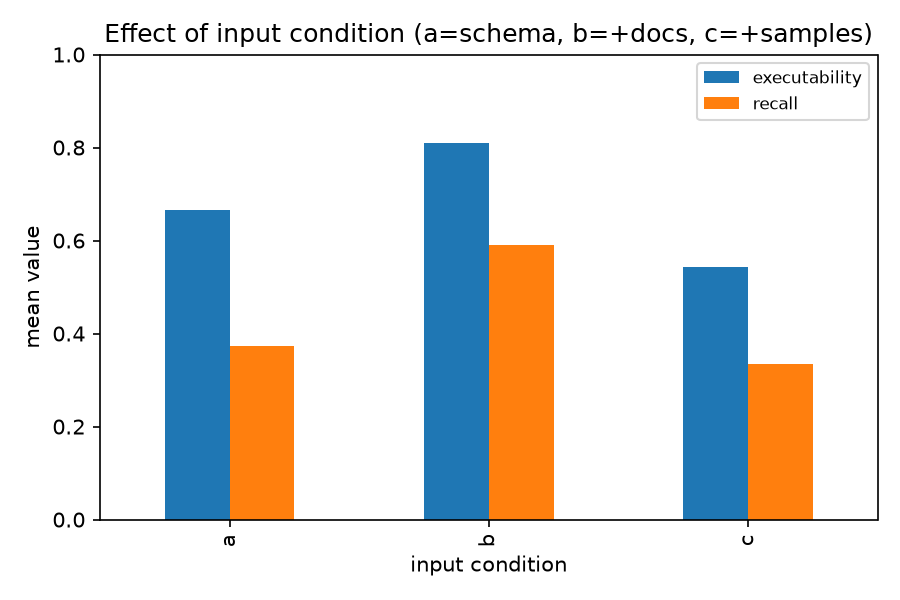
\includegraphics[width=\linewidth]{figures/condition_comparison.png}
\caption{Condition comparison (RQ3): documentation helps, sample rows hurt.}
\label{fig:cond}
\end{figure}

\subsection{RQ4: Model choice and cost}
Among local models the 32B code model dominates every quality axis
(Tables~\ref{tab:exec}--\ref{tab:bytype}) but at a cost: mean generation latency
is $\approx\!100$\,s per suite versus $15$--$18$\,s for the 7--8B models (a
$5$--$7\times$ gap), and it emits the most completion tokens ($\approx\!930$ vs.\
510--680). For a build-time, cacheable artifact this latency is easily
amortized---every call in our study is cached---so the quality gain is worth
paying for. The smaller models are not merely weaker but qualitatively risky:
\texttt{llama3.1-8b}'s 51\% clean-row false-positive rate would bury real signal
under noise in production.

\begin{figure}[t]
\centering
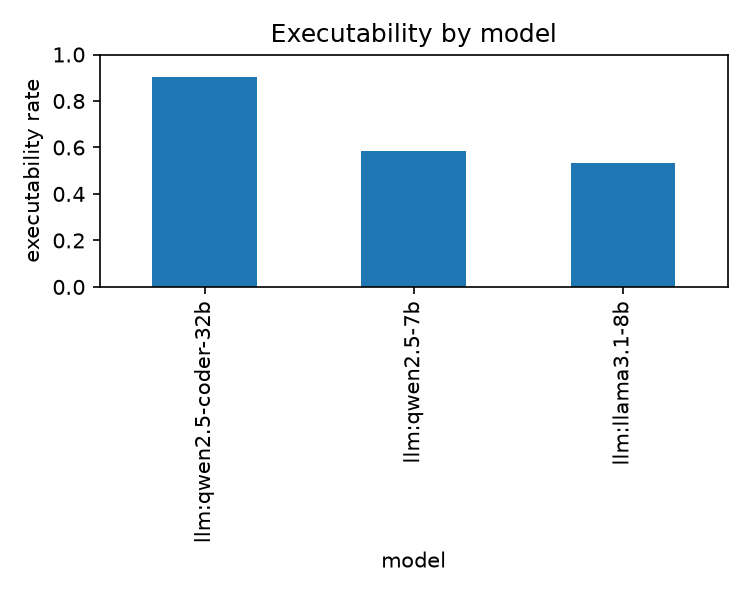
\includegraphics[width=\linewidth]{figures/executability_by_model.png}
\caption{Executability by model (RQ4). Scale and code specialization both help.}
\label{fig:exec}
\end{figure}

% ===========================================================================
\section{Discussion}\label{sec:discussion}
% ===========================================================================
\paragraph{LLMs as a breadth-first drafter, not a replacement.}
The honest headline is that today's local open-weight models do not beat a good
statistical profiler or a careful hand-written suite on raw detection. Their
value is elsewhere: a single 32B model, from documentation alone, produces an
executable suite that spans range, domain, type, and \emph{cross-column} checks
in one pass---covering ground that profiling (no cross-column reasoning) and
quick hand-rules (incomplete coverage) each miss. The natural deployment is
\emph{LLM-drafts-then-human-prunes}, or an ensemble in which the LLM supplies
cross-column and semantic checks on top of a profiler's range checks.

\paragraph{Executability is a first-class gate.}
Detection quality is meaningless if the suite does not run. The 32B/8B gap in
executability (0.90 vs.\ 0.53) and especially the small models' clean-data false
positives argue for the allowlist-plus-parse-validate design as mandatory
scaffolding, not an optimization.

\paragraph{Less context can be more.}
The RQ3 reversal from sample rows is a concrete, actionable result: documentation
generalizes, instances over-fit. Prompt designers for data-tooling should prefer
semantic description over data samples.

% ===========================================================================
\section{Threats to Validity}\label{sec:threats}
% ===========================================================================
\textbf{Construct.} Row-level recall depends on the injection design; our rates,
seeds, and target columns are fixed and released, but other error distributions
could shift the per-type picture. The referential-integrity measurement is a
single-table artifact (see RQ2). \textbf{Internal.} We run temperature~0 with one
repetition in this medium-scope configuration; the pipeline supports multiple
repetitions and seeds for variance estimation, which we leave for a full-scale
run. Large-table detection uses fixed-seed subsampling for per-row error types,
which is unbiased in expectation but adds sampling variance. \textbf{External.} We
study three local open-weight models and two datasets; frontier API models and
other domains may behave differently. The pipeline includes API backends behind a
config flag precisely so RQ4 can be extended to close the local-vs-API gap.

% ===========================================================================
\section{Related Work}\label{sec:related}
% ===========================================================================
Automated data-quality verification frameworks such as
Deequ~\cite{amazondeequ} and Great Expectations~\cite{greatexpectations} provide
the execution substrate but assume constraints are authored by humans or mined
statistically. Empirical treatments of data quality~\cite{dataqualitysurvey}
emphasize that constraint elicitation is the practical bottleneck. Recent work
asks whether foundation models can perform data-management tasks such as
imputation and entity matching~\cite{llmdataeng}; we specialize that question to
\emph{constraint generation} and, crucially, measure executability and
controlled detection rather than task accuracy alone.

% ===========================================================================
\section{Conclusion}
% ===========================================================================
We studied whether LLMs can draft runnable data-quality constraints from schema
and documentation. With an allowlist-constrained, validate-everything pipeline, a
32B code model reaches 0.90 executability and produces the most \emph{balanced}
detector among all methods---uniquely combining cross-column and range/domain
coverage---though classical baselines still win on raw aggregate detection.
Documentation is the dominant prompt ingredient and sample rows are
counterproductive. The results point to a human-in-the-loop or ensemble
deployment in which the LLM contributes breadth. All code, prompts, and the
injection benchmark are released for reproduction.

\bibliographystyle{plain}
\bibliography{references}

\end{document}
